
\section{Recuperação de chaves com erros em criptosistemas baseados no (EC)DLP}

%Due to noise, data leakage (note that we are aiming at exploiting the address leakage only), and other aspects that interfere with the side-channel analysis (misalignment, clock jitter, etc), the derivation of the final scalar for a single trace likely contains errors. 
%
Devido ao ruído, vazamento de dado (por canal lateral) não relacionado à chave secreta, e outros aspectos que interferem com a análise por canal lateral (p.ex., desalinhamento, clock jitter), o escalar final obtido por ataque SCA realizado a partir de um único trace provavelmente conterá erros, isto é, o valor de alguns dos bits recuperados estará incorreto.

%
%If the amount of wrong bits is sufficiently small, then a brute-force attack may still be feasible. 
%
Se a quantidade de bits incorretos (erros) é suficientemente pequena, então um ataque de força bruta pode ser viável, mesmo que não se saiba a localização de tais bits incorretos. A complexidade de tal busca, isto é, o número de escalares que devem ser testados até o escalar correto ser encontrado é ${{n}\choose{s}} 2^s$, onde $n$ é o comprimento do escalar em bits e $s$ é número de erros. Considerando um escalar de $n = 256$ bits\footnote{comprimento típico do escalar para uma curva no nível de segurança de 128 bits}, o valor máximo de $s$ para concluir tal busca em tempo aceitável é 6, o que significa que aproximadamente $2^{56}$ escalares precisam ser testados.

%
% However, first the attacker needs a metric to indicate the location of the possible wrong bits in the recovered scalar. 
%
Se a quantidade de bits incorretos for maior, então o atacante necessita saber a localização dos possíveis bits incorretos nos escalar recuperado para corrigi-los em tempo viável.
%
% The notion of suspicious bits (cf.~\Cref{cswap-arith-template-gen-and-match}) can be used as a reference for the scalar bits selection with respect to a brute-force attack. 
%
Neste caso, a noção de bits suspeitos\erick{definir} pode ser usada como referência para a seleção de bits do escalar com respeito a um ataque de força bruta.
%

\newcommand{\iterations}{254}

% Let us consider the trace with smallest amount of suspicious bits from the experiment from (Section\erick{ref. Section load attack SAC2016}} as an example; for this trace there are $\iterations$ suspicious bits that comprise all falsely identified bits.
%%%
%TODO
%%%
% Unfortunately, to recover a full randomized scalar, even in this case, the attacker needs $O(2^{\iterations})$ operations, which is generally impractical. 
%%%
%TODO
%%%
% Note, that we consider only the worst-case complexity and not the average case. 
%%%
%TODO
%%%
% To improve the brute-force complexity, there are two options.
%%%
%TODO
%%%
% The first approach is to try to exploit the distribution of suspicious bits for incorrectly (red) and correctly (blue) recovered bits (\Cref{fig:hist-conf-all-traces__n_trset_40}). While there is a clear trend for incorrect bits to have lower confidence score, the intersection between correct and incorrect bits is large. 
%%%
%TODO
%%%
% Still, it may possible to exploit the trend with an informed brute force attack~\cite{kang2014}, prioritizing bits with the lowest confidence score.
%%%
%TODO
%%%
% Unfortunately this attack works well if the bits containing errors are adjacent and that is not the case in our setting. 
%%%
%TODO
%%%

\begin{figure}[h!tb]
	\centering   %height=0.20\textheight
	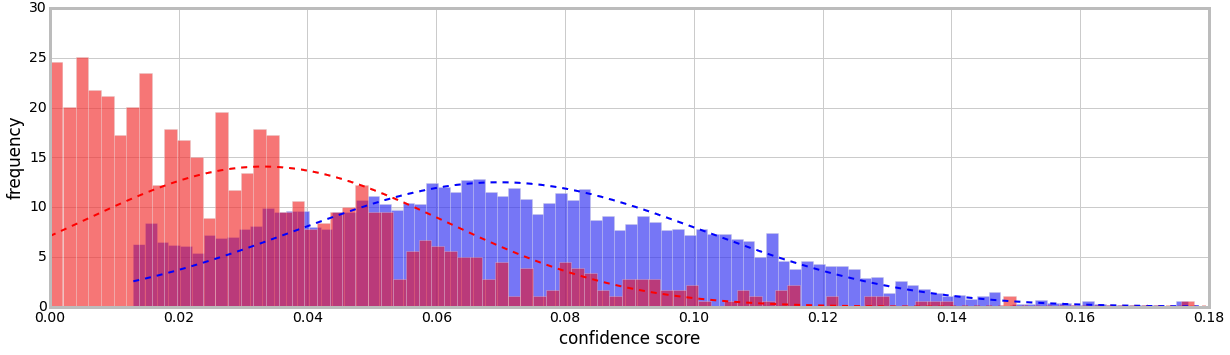
\includegraphics[width=0.9\textwidth]{figures/SAC_2016__pointer_cswap_attack__hist-conf-all-traces__n_trset_40.png}
	\caption{Distribution of confidence scores over all traces for suspicious bits. Red: incorrectly recovered bits, blue: correctly recovered but suspicious bits.}
	\vspace{.5mm}
	\label{fig:hist-conf-all-traces__n_trset_40}
\end{figure}

\subsection{Algoritmo de Gopalakrishnan, Theriault e Yao~\cite{GopalakrishnanTheriaultYao07}}
%\erick[inline]{copiar texto do paper SAC. Baseado no paradigma time-memory trade-off}
%%%
%TODO
%%%
% Alternatively (or combined with the informed brute-force search), we apply the second algorithm from~\cite{chain_recovery_2007}, which is originally designed for \emph{square-and-multiply chains}, to the Montgomery ladder. 
%%%
%TODO
%%%
% We describe how the algorithm works using the aforementioned example trace,  which contains $s=\iterations$ suspicious bits, as an example. Let us represent the indices of these bits as a list sorted in descending order: $i_s, \dots i_1$, 
%%%
%TODO
%%%
% where each $i_j \in \{0, \dots 254\}$ and $s \ge j \ge 1$; note that there are $255$~bits in total. Let $x$ denote the bit index $i_{\floor*{\frac{s}{2} + 1}}$ (namely, $i_{\x}$ for the example trace). 
%%%
%TODO
%%%
%Let $a$ be the number represented by the bit string corresponding to the left part of the scalar from $x$ (including $i_x$) and let $b$ be the number corresponding to the bit string of the (least significant) right part.
%let $y=254-i_x$ be the length of the right part. 
%Furthermore, we know that $R = [k] P$, 
%%%
%TODO
%%%
%where $R$ is the resulting point, $k$ the scalar to be recovered, 
% and $P$ the input point. 
%%%
%TODO
%%%
% Then, clearly 
%\begin{equation*}
% $R = [k] P = [a \cdot 2^{i_x} + b] P = [a] ([2^{i_x}] P) + [b] P$. 
%\end{equation*}
%%%
%TODO
%%%
% If we denote $[2^{i_x}] P$ by $H$, then the above equation reduces to
% \begin{equation}\label{eq:check}
% R - [b] P = [a] H
% \end{equation}
%%%
%TODO
%%%

\subsection{Aplicação do Algoritmo de Gopalakrishnan, Theriault e Yao~\cite{GopalakrishnanTheriaultYao07} à curva elíptica Curve25519}

\erick[inline]{Explicar as otimizações de desempenho que podem ser aplicadas à nível de aritmética na curva}


\begin{comment}
%\subsection{Algoritmo de Lange, Vrendendaal e Wakker~\cite{LangeVredendaalWakker2014}}
%\erick[inline]{baseado no algoritmo de Pollard-Kangaroo. Utilizar texto da discussão por email com os autores.}
\end{comment}